\documentclass{beamer}

\mode<presentation> {

% The Beamer class comes with a number of default slide themes
% which change the colors and layouts of slides. Below this is a list
% of all the themes, uncomment each in turn to see what they look like.


\usetheme{default}
%\usetheme{AnnArbor}
%\usetheme{Antibes}
%\usetheme{Bergen}
%\usetheme{Berkeley}
%\usetheme{Berlin}
%\usetheme{Boadilla}
%\usetheme{CambridgeUS}
%\usetheme{Copenhagen}
%\usetheme{Darmstadt}
%\usetheme{Dresden}
%\usetheme{Frankfurt}
%\usetheme{Goettingen}
%\usetheme{Hannover}
%\usetheme{Ilmenau}
%\usetheme{JuanLesPins}
%\usetheme{Luebeck}
%\usetheme{Madrid}
%\usetheme{Malmoe}
%\usetheme{Marburg}
%\usetheme{Montpellier}
%\usetheme{PaloAlto}
%\usetheme{Pittsburgh}
%\usetheme{Rochester}
%\usetheme{Singapore}
%\usetheme{Szeged}
%\usetheme{Warsaw}

% As well as themes, the Beamer class has a number of color themes
% for any slide theme. Uncomment each of these in turn to see how it
% changes the colors of your current slide theme.

%\usecolortheme{albatross}
%\usecolortheme{beaver}
%\usecolortheme{beetle}
%\usecolortheme{crane}
%\usecolortheme{dolphin}
%\usecolortheme{dove}
%\usecolortheme{fly}
%\usecolortheme{lily}
%\usecolortheme{orchid}
%\usecolortheme{rose}
%\usecolortheme{seagull}
%\usecolortheme{seahorse}
%\usecolortheme{whale}
%\usecolortheme{wolverine}

%\setbeamertemplate{footline} % To remove the footer line in all slides uncomment this line
\setbeamertemplate{footline}[page number] % To replace the footer line in all slides with a simple slide count uncomment this line

\setbeamertemplate{navigation symbols}{} % To remove the navigation symbols from the bottom of all slides uncomment this line
}

\usepackage{graphicx}
\usepackage{booktabs}
\usepackage{amssymb}
\usepackage{color}
\usepackage{subcaption}
\usepackage{caption}
\usepackage{float}



\AtBeginSection[]{
  \begin{frame}
  \vfill
  \centering
  \begin{beamercolorbox}[sep=8pt,center,shadow=true,rounded=true]{title}
    \usebeamerfont{title}\insertsectionhead\par%
  \end{beamercolorbox}
  \vfill
  \end{frame}
}


\title{Image Inpainting Software}

\author{Team 27: Yesheng Ma\\\hspace{0.9cm}Hu Hu\\\hspace{1.4cm}Yikai Zou}
\institute[SJTU]{}
\date{\today}

\begin{document}

\begin{frame}
\titlepage
\end{frame}



\section{Introduction}


\section{Existing Approaches}


\section{Proposed Ideas and Implementation}
\subsection{Markov Random Field}

\subsection{Exemplar-Based Algorithm}
\begin{frame}{Exemplar-Based Algorithm}
	\textbf{Observations:}
	\begin{itemize}[<+->]
		\item Using single pix as basic unit will result in blurry. \\So we using patch (i.e. 3x3) as basic unit.
		\item In-painting order is important for final result. 
		\begin{figure}
			\centering
			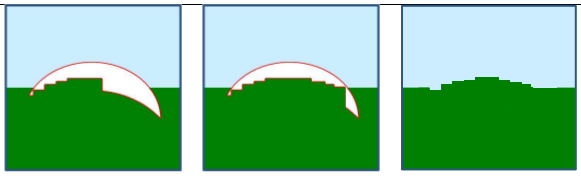
\includegraphics[width=0.8\linewidth]{order1.png}\\
			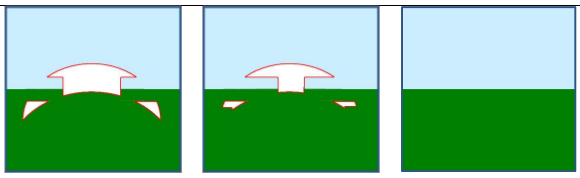
\includegraphics[width=0.8\linewidth]{order2.png}
			\caption{In-painting by different order}
		\end{figure}
	\end{itemize}
\end{frame}

\begin{frame}{Exemplar-Based Algorithm}
	\textbf{In-painting Process:}
	\begin{itemize}[<+->]
		\item Patch selection: We need to select the specific patch to in-paint first. We define the priority function:
		\begin{equation*}
		\centering
		P(p)=C(p)*D(p)
		\nonumber
		\end{equation*}
		where: $C(p)=\frac{\sum_{q\in \Phi _p\cap(-\Omega)}*C(q)}{|\Phi_p|}$, $D(p)=\frac{|\nabla I^\bot_p \cdot n_p|}{\alpha}$.
		\item During each loop, we calculate the C(p) and D(p) of each patch, choose the patch with maximum priority.
		\item Then we find the exemplar patch that minimize the Euclidean distance between them and in-paint the former patch.
		\item We implemented this algorithm in python.
	\end{itemize}
\end{frame}


\section{Demo}
\begin{frame}{Demo}
	\begin{itemize}
		\item Using Markov random filed algorithm:
		\begin{figure}
			\centering
			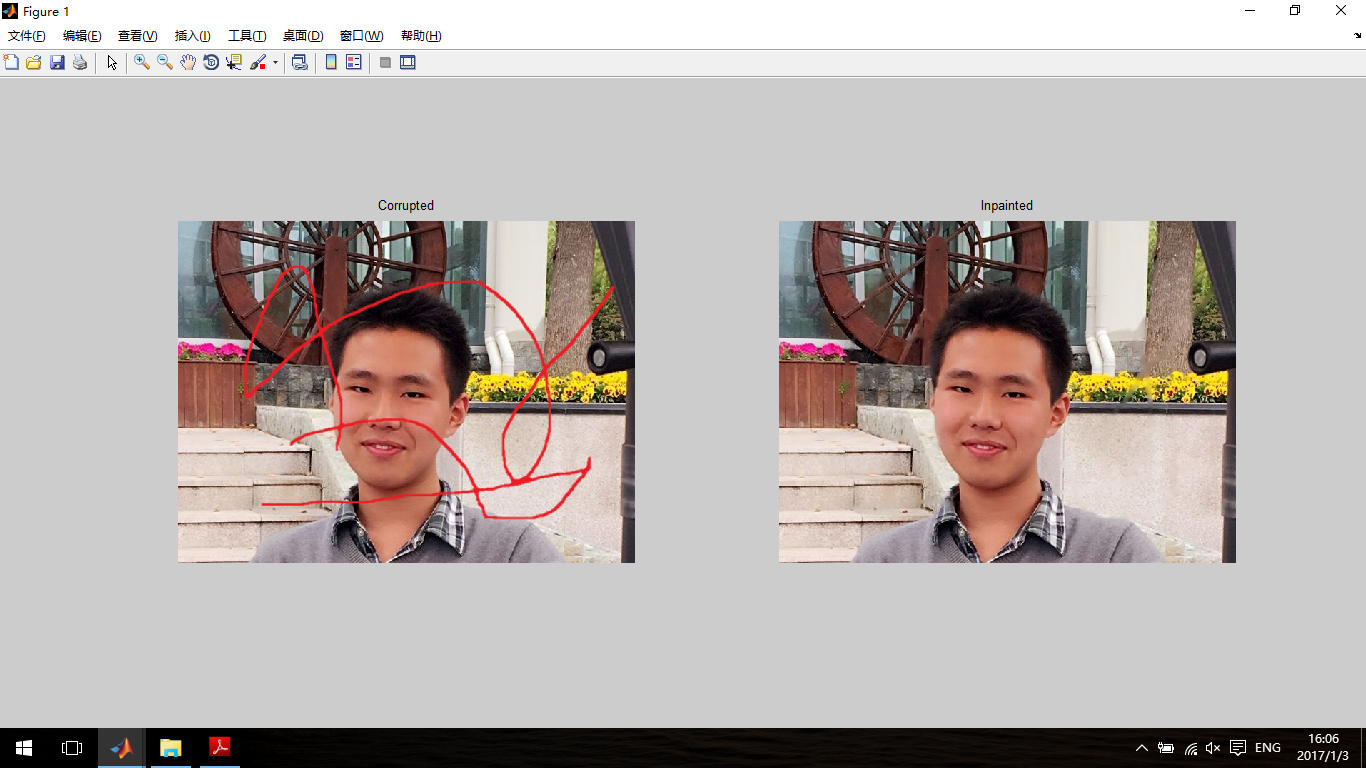
\includegraphics[width=1.0\linewidth]{rmf_result.png}
			\caption{Result by MRF Implementation}
		\end{figure}
	\end{itemize}
\end{frame}

\begin{frame}{Demo}
	\begin{itemize}
		\item Using exemplar-based algorithm:
		\begin{figure}
			\centering
			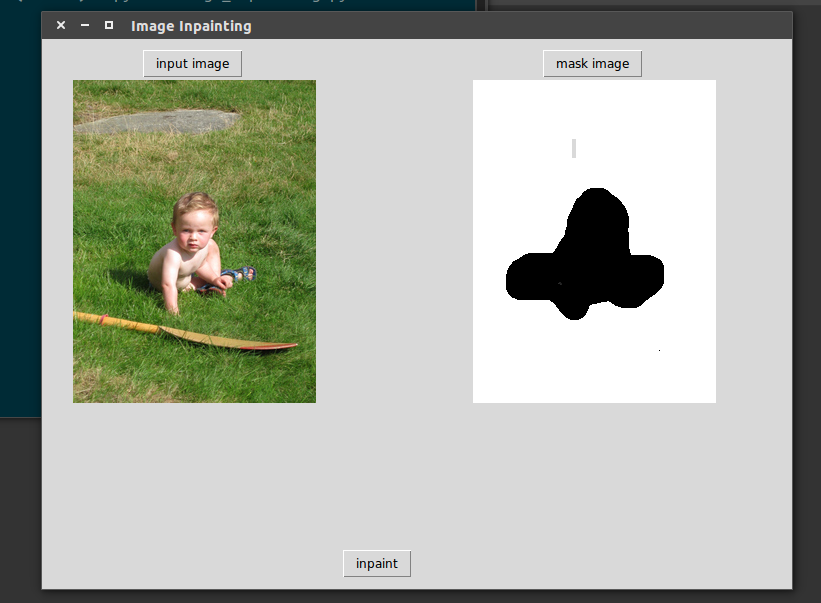
\includegraphics[width=0.8\linewidth]{eb_result.png}
			\caption{Result by exemplar-based Implementation}
		\end{figure}
	\end{itemize}
\end{frame}

\begin{frame}{Demo}
	\begin{itemize}
		\item Using exemplar-based algorithm (Con'd)
		\begin{figure}
			\begin{subfigure}[pos]{.5\textwidth}
				\centering
				\includegraphics*[width=0.6\linewidth]{in1.jpg}
				\caption{Original picture}
			\end{subfigure}%
			\begin{subfigure}[pos]{.5\textwidth}
				\centering
				\includegraphics*[width=0.6\linewidth]{out1.jpg}
				\caption{In-painted picture}
			\end{subfigure}%
			\caption{Result by exemplar-based Implementation}
		\end{figure}
	\end{itemize}
\end{frame}


\section{Conclusion and Future Work}
\begin{frame}{Conclusion and Future Work}
	\begin{itemize}[<+->]
		\item We accomplished the chosen task and solved the problem. The result works well.
		\item The proposed ideas given by us successfully solve the Image In-painting problem.\\\ \\
		\item In this AI age, we plan to apply deep learning model in this topic in the future. We have designed the network structure for image in-painting. If we get enough data one day, we will try this deep learning model on this topic.
	\end{itemize}
\end{frame}

\section*{Reference}
\begin{frame}{Reference}
	\begin{itemize}
		\item M. Bertalmio, G. Sapiro, V. Caselles, and C. Ballester, Image in-painting, in $Proc.\ SIGGRAPH$, 2000, pp. 417-424
		\item S. Roth and M. J. Black. Fields of experts. $IJCV$, 82(2):205–229,
		2009.
		\item A. Criminisi, P. Perez, and K. Toyama, Region filling and object
		removal by examplar-based image inpainting, IEEE $Trans. Image\ 
		Process.$, vol. 13, pp. 1200-1212, 2004.
		\item G. E. Hinton. Training products of experts by minimizing contrastive
		divergence. $Neural\ Comput.$, 14(8):1771-1800, 2002.
		\item M. Welling, G. E. Hinton, and S. Osindero. Learning sparse to-
		pographic representations with products of Student-t distributions.
		$NIPS*2002$.
	\end{itemize}
\end{frame}

%\begin{frame}
%\frametitle{Overview}
%\tableofcontents
%\end{frame}

%\section{Introduction}
%\begin{frame}
%\frametitle{Prisoner's Dilemma}
%Prisoner's Dilemma:\\
%\begin{itemize}[<+->]
%\item
%\begin{tabular}{|c|c|c|}
%\hline
%\hline
%    &{\color{red}Alice} Deny&{\color{red}Alice} Confess\\
%\hline
%{\color{blue}Bob} Deny& ({\color{blue}-1},{\color{red}-1}) & ({\color{blue}-9},{\color{red}0})\\
%\hline
%{\color{blue}Bob} Confess& ({\color{blue}0},{\color{red}-9}) & ({\color{blue}-6},{\color{red}-6})\\
%\hline
%\hline
%\end{tabular}
%\item
%{\color{blue}$S_B = \{ C, D\}$}  \qquad {\color{red}$S_A = \{ C, D\}$}
%\item
%{\color{blue}$u_B(D,{\color{red}D}) = -1$} \qquad {\color{red}$u_A({\color{blue}D},D) = -1$}
%\item
%{\color{blue}$u_B(D,{\color{red}C}) = -9$} \qquad {\color{red}$u_A({\color{blue}D},C) = 0$}\\
%{\color{blue}$u_B(C,{\color{red}D}) = 0 $} \text{ } \qquad {\color{red}$u_A({\color{blue}C},D) = -9$}\\
%{\color{blue}$u_B(C,{\color{red}C}) = -6$} \qquad {\color{red}$u_A({\color{blue}C},C) = -6$}
%\end{itemize}
%\end{frame}
%
%\begin{frame}
%\frametitle{What is a Non-zero Sum Game?}
%\begin{itemize}
%\item
%The sum of each player's gain or loss $\neq$ what they begin with.
%\item
%$\exists (s_1,s_2,...,s_n)\in S_1\times S_2 \times ... \times S_n$, $\sum_{i=1}^{n} u_i(s_1,s_2,...,s_n) \neq 0$
%\end{itemize}
%\end{frame}
%
%\begin{frame}
%\frametitle{Strict Domination}
%Assuming you are {\color{blue}Bob}, what should you do?\\
%\begin{itemize}[<+->]
%\item
%\begin{tabular}{|c|c|c|}
%\hline
%\hline
%    &{\color{red}Alice} Deny&{\color{red}Alice} Confess\\
%\hline
%{\color{blue}Bob} Deny& ({\color{blue}-1},{\color{red}-1}) & ({\color{blue}-9},{\color{red}0})\\
%\hline
%{\color{blue}Bob} Confess& ({\color{blue}0},{\color{red}-9}) & ({\color{blue}-6},{\color{red}-6})\\
%\hline
%\hline
%\end{tabular}
%
%\item
%What if {\color{red}Alice} chooses to \textbf{Deny}?
%\item
%Result: {\color{blue}Bob} is free and {\color{red}Alice} will spend 9 years.
%\item
%What if {\color{red}Alice} chooses to \textbf{Confess}?
%\item
%Result: {\color{blue}Bob} and {\color{red}Alice} will spend 6 years together.
%\item
%\textbf{In both cases, }{\color{blue}Bob}\textbf{ will definitely choose to confess.}
%\end{itemize}
%\end{frame}
%
%\begin{frame}
%\frametitle{Strict Domination}
%The process is like:\\
%\centering
%\begin{tabular}{|c|c|c|}
%\hline
%\hline
%    &{\color{red}Alice} Deny&{\color{red}Alice} Confess\\
%\hline
%{\color{blue}Bob} Deny& ({\color{blue}-1},{\color{red}-1}) & ({\color{blue}-9},{\color{red}0})\\
%\hline
%{\color{blue}Bob} Confess& ({\color{blue}0},{\color{red}-9}) & ({\color{blue}-6},{\color{red}-6})\\
%\hline
%\hline
%\end{tabular}
%\end{frame}
%
%\begin{frame}
%\frametitle{Strict Domination}
%The process is like:\\
%\centering
%\begin{tabular}{|c|c|c|}
%\hline
%\hline
%    &{\color{red}Alice} Deny&{\color{red}Alice} Confess\\
%\hline
%{\color{blue}Bob} Deny& ({\color{blue}-1},{\color{red}-1}) & ({\color{blue}-9},{\color{red}0})\\
%\hline
%{\color{blue}Bob} Confess& ({\color{blue}0},{\color{red}-9}) & ({\color{blue}-6},{\color{red}-6})\\
%\hline
%\hline
%\end{tabular}\\
%$\Downarrow$\\
%\begin{tabular}{|c|c|c|}
%\hline
%\hline
%    &{\color{red}Alice} Deny&{\color{red}Alice} Confess\\
%\hline
%{\color{blue}Bob} Confess& ({\color{blue}0},{\color{red}-9}) & ({\color{blue}-6},{\color{red}-6})\\
%\hline
%\hline
%\end{tabular}\\
%\end{frame}
%
%\begin{frame}
%\frametitle{Strict Domination}
%The process is like:\\
%\centering
%\begin{tabular}{|c|c|c|}
%\hline
%\hline
%    &{\color{red}Alice} Deny&{\color{red}Alice} Confess\\
%\hline
%{\color{blue}Bob} Deny& ({\color{blue}-1},{\color{red}-1}) & ({\color{blue}-9},{\color{red}0})\\
%\hline
%{\color{blue}Bob} Confess& ({\color{blue}0},{\color{red}-9}) & ({\color{blue}-6},{\color{red}-6})\\
%\hline
%\hline
%\end{tabular}\\
%$\Downarrow$\\
%\begin{tabular}{|c|c|c|}
%\hline
%\hline
%    &{\color{red}Alice} Deny&{\color{red}Alice} Confess\\
%\hline
%{\color{blue}Bob} Confess& ({\color{blue}0},{\color{red}-9}) & ({\color{blue}-6},{\color{red}-6})\\
%\hline
%\hline
%\end{tabular}\\
%$\Downarrow$\\
%\begin{tabular}{|c|c|c|}
%\hline
%\hline
%    &{\color{red}Alice} Confess\\
%\hline
%{\color{blue}Bob} Confess& ({\color{blue}-6},{\color{red}-6})\\
%\hline
%\hline
%\end{tabular}\\
%\end{frame}
%
%\begin{frame}
%\frametitle{Strict Domination}
%\begin{itemize}[<+->]
%\item
%If one of the player’s strategies is never the right thing to do, no matter what the opponents do, it is \textbf{Strictly Dominated}.
%\item
%Get rid of the strictly dominated strategies because \textbf{they won't happen}.
%\item
%This is called \textbf{iterated elimination of dominated strategies}.
%\end{itemize}
%\end{frame}
%
%
%\section{Mixed Strategy Example}
%\begin{frame}
%\frametitle{Bob and Alice}
%\begin{itemize}
%\item {\color{blue}Bob} and {\color{red} Alice} are students in some school.
%\item {\color{blue}Bob} loves {\color{red} Alice} but {\color{red} Alice} dont like {\color{blue}Bob}.
%\item The situation arises when they decide where to eat lunch.
%\end{itemize}
%\end{frame}
%
%\begin{frame}
%\frametitle{Restaurant}
%\begin{itemize}
%\item Restaurant No.1's food is awful.
%\item Restaurant No.3's food is better.
%\end{itemize}
%
%\end{frame}
%
%\begin{frame}
%\frametitle{Their Pay-off when eating}
%\begin{tabular}{|c|c|c|}
%\hline
%\hline
%    & {\color{red}Alice} go to No.3 & {\color{red}Alice} go to No.1\\
%\hline
%{\color{blue}Bob} go to No.3 & ({\color{blue}10},{\color{red}4}) & \\
%\hline
%{\color{blue}Bob} go to No.1 &  & \\
%\hline
%\hline
%\end{tabular}
%\end{frame}
%
%\begin{frame}
%\frametitle{Their Pay-off when eating}
%\begin{tabular}{|c|c|c|}
%\hline
%\hline
%    & {\color{red}Alice} go to No.3 & {\color{red}Alice} go to No.1\\
%\hline
%{\color{blue}Bob} go to No.3 & ({\color{blue}10},{\color{red}4}) & ({\color{blue}3},{\color{red}5})\\
%\hline
%{\color{blue}Bob} go to No.1 &  & \\
%\hline
%\hline
%\end{tabular}
%\end{frame}
%
%\begin{frame}
%\frametitle{Their Pay-off when eating}
%\begin{tabular}{|c|c|c|}
%\hline
%\hline
%    & {\color{red}Alice} go to No.3 & {\color{red}Alice} go to No.1\\
%\hline
%{\color{blue}Bob} go to No.3 & ({\color{blue}10},{\color{red}4}) & ({\color{blue}3},{\color{red}5})\\
%\hline
%{\color{blue}Bob} go to No.1 & ({\color{blue}0},{\color{red}10}) & \\
%\hline
%\hline
%\end{tabular}
%\end{frame}
%
%\begin{frame}
%\frametitle{Their Pay-off when eating}
%\begin{tabular}{|c|c|c|}
%\hline
%\hline
%    & {\color{red}Alice} go to No.3 & {\color{red}Alice} go to No.1\\
%\hline
%{\color{blue}Bob} go to No.3 & ({\color{blue}10},{\color{red}4}) & ({\color{blue}3},{\color{red}5})\\
%\hline
%{\color{blue}Bob} go to No.1 & ({\color{blue}0},{\color{red}10}) & ({\color{blue}7},{\color{red}0})\\
%\hline
%\hline
%\end{tabular}
%\end{frame}
%
%\begin{frame}
%\frametitle{How will they act?}
%\begin{tabular}{|c|c|c|}
%\hline
%\hline
%    & {\color{red}Alice} go to No.3 & {\color{red}Alice} go to No.1\\
%\hline
%{\color{blue}Bob} go to No.3 & ({\color{blue}10},{\color{red}4}) {\color{green}*}& ({\color{blue}3},{\color{red}5})\\
%\hline
%{\color{blue}Bob} go to No.1 & ({\color{blue}0},{\color{red}10}) & ({\color{blue}7},{\color{red}0})\\
%\hline
%\hline
%\end{tabular}
%\begin{itemize}
%\item
%If {\color{blue}Bob} claims in WeChat that he will go to No.3 and {\color{red}Alice} claims that she will go to No.3.
%
%\item What will happen?
%\end{itemize}
%\end{frame}
%
%\begin{frame}
%\frametitle{How will they act?}
%\begin{tabular}{|c|c|c|}
%\hline
%\hline
%    & {\color{red}Alice} go to No.3 & {\color{red}Alice} go to No.1\\
%\hline
%{\color{blue}Bob} go to No.3 & ({\color{blue}10},{\color{red}4})& ({\color{blue}3},{\color{red}5})  {\color{green}*}\\
%\hline
%{\color{blue}Bob} go to No.1 & ({\color{blue}0},{\color{red}10}) & ({\color{blue}7},{\color{red}0})\\
%\hline
%\hline
%\end{tabular}
%\begin{itemize}
%\item {\color{red}Alice} will choose to go to No.3 restaurant.
%\end{itemize}
%\end{frame}
%
%\begin{frame}
%\frametitle{How will they act?}
%\begin{tabular}{|c|c|c|}
%\hline
%\hline
%    & {\color{red}Alice} go to No.3 & {\color{red}Alice} go to No.1\\
%\hline
%{\color{blue}Bob} go to No.3 & ({\color{blue}10},{\color{red}4})& ({\color{blue}3},{\color{red}5})\\
%\hline
%{\color{blue}Bob} go to No.1 & ({\color{blue}0},{\color{red}10}) & ({\color{blue}7},{\color{red}0}) {\color{green}*}\\
%\hline
%\hline
%\end{tabular}
%\begin{itemize}
%\item Then {\color{blue}Bob} will choose to go to No.3 restaurant.
%\end{itemize}
%\end{frame}
%
%\begin{frame}
%\frametitle{How will they act?}
%\begin{tabular}{|c|c|c|}
%\hline
%\hline
%    & {\color{red}Alice} go to No.3 & {\color{red}Alice} go to No.1\\
%\hline
%{\color{blue}Bob} go to No.3 & ({\color{blue}10},{\color{red}4})& ({\color{blue}3},{\color{red}5}) \\
%\hline
%{\color{blue}Bob} go to No.1 & ({\color{blue}0},{\color{red}10}) {\color{green}*} & ({\color{blue}7},{\color{red}0})\\
%\hline
%\hline
%\end{tabular}
%\begin{itemize}
%\item Then {\color{red}Alice} will choose to go to No.3 restaurant.
%\end{itemize}
%\end{frame}
%
%\begin{frame}
%\frametitle{How will they act?}
%\begin{tabular}{|c|c|c|}
%\hline
%\hline
%    & {\color{red}Alice} go to No.3 & {\color{red}Alice} go to No.1\\
%\hline
%{\color{blue}Bob} go to No.3 & ({\color{blue}10},{\color{red}4}) {\color{green}*}& ({\color{blue}3},{\color{red}5})\\
%\hline
%{\color{blue}Bob} go to No.1 & ({\color{blue}0},{\color{red}10}) & ({\color{blue}7},{\color{red}0})\\
%\hline
%\hline
%\end{tabular}
%\begin{itemize}
%\item Then {\color{blue}Bob} will choose to go to No.3 restaurant.
%\item {\Large It is a circulation!!}
%\end{itemize}
%\end{frame}
%
%\begin{frame}
%\frametitle{What should they do?}
%\begin{tabular}{|c|c|c|}
%\hline
%\hline
%    & {\color{red}Alice} go to No.3 & {\color{red}Alice} go to No.1\\
%\hline
%{\color{blue}Bob} go to No.3 & ({\color{blue}10},{\color{red}4}) & ({\color{blue}3},{\color{red}5})\\
%\hline
%{\color{blue}Bob} go to No.1 & ({\color{blue}0},{\color{red}10}) & ({\color{blue}7},{\color{red}0})\\
%\hline
%\hline
%\end{tabular}
%\begin{itemize}
%\item When the two persons are stuck in this dilemma, a third person comes out and say, {\Large "Why don't you just choose the restaurant by probability?}"
%\item That's it!
%\end{itemize}
%\end{frame}
%
%\begin{frame}
%\frametitle{What should they do?}
%\begin{tabular}{|c|c|c|}
%\hline
%\hline
%    & {\color{red}Alice} go to No.3 & {\color{red}Alice} go to No.1\\
%\hline
%{\color{blue}Bob} go to No.3 & ({\color{blue}10},{\color{red}4}) & ({\color{blue}3},{\color{red}5})\\
%\hline
%{\color{blue}Bob} go to No.1 & ({\color{blue}0},{\color{red}10}) & ({\color{blue}7},{\color{red}0})\\
%\hline
%\hline
%\end{tabular}
%\begin{itemize}
%\item Supposed that Alice will choose No.3 by probability $a_1$ and choose No.1 by $a_2$.
%\end{itemize}
%\end{frame}
%
%\begin{frame}
%\frametitle{What should they do?}
%\begin{tabular}{|c|c|c|}
%\hline
%\hline
%    & {\color{red}Alice} go to No.3 & {\color{red}Alice} go to No.1\\
%\hline
%{\color{blue}Bob} go to No.3 & ({\color{blue}10},{\color{red}4}) & ({\color{blue}3},{\color{red}5})\\
%\hline
%{\color{blue}Bob} go to No.1 & ({\color{blue}0},{\color{red}10}) & ({\color{blue}7},{\color{red}0})\\
%\hline
%\hline
%\end{tabular}
%\begin{itemize}
%\item Supposed that Alice will choose No.3 by probability $a_1$ and choose No.1 by $a_2$.
%\item Then if Bob go to No.3, his pay-off will be $10a_1+3a_2$. If he go to No.1, then pay-off will be $7a_2$.
%\end{itemize}
%\end{frame}
%
%\begin{frame}
%\frametitle{What should they do?}
%\begin{tabular}{|c|c|c|}
%\hline
%\hline
%    & {\color{red}Alice} go to No.3 & {\color{red}Alice} go to No.1\\
%\hline
%{\color{blue}Bob} go to No.3 & ({\color{blue}10},{\color{red}4}) & ({\color{blue}3},{\color{red}5})\\
%\hline
%{\color{blue}Bob} go to No.1 & ({\color{blue}0},{\color{red}10}) & ({\color{blue}7},{\color{red}0})\\
%\hline
%\hline
%\end{tabular}
%\begin{itemize}
%\item Supposed that Alice will choose No.3 by probability $a_1$ and choose No.1 by $a_2$.
%\item Then if Bob go to No.3, his pay-off will be $10a_1+3a_2$. If he go to No.1, then pay-off will be $7a_2$.
%\item $10a_1+3a_2$ must be equal to $7a_2$, otherwise Bob can decide indeed which restaurant to go. And it will be circulation again.\\
%\end{itemize}
%\end{frame}
%
%\begin{frame}
%\frametitle{What should they do?}
%        \qquad $10a_1+3a_2$ = $7a_2$ \\
%        \qquad $a_1 + a_2 = 1$ \\
%        \qquad So $a_1 = \frac{2}{7}, a_2 = \frac{5}{7}$
%\end{frame}
%
%
%\begin{frame}
%\frametitle{What should they do?}
%\begin{tabular}{|c|c|c|}
%\hline
%\hline
%    & {\color{red}Alice} go to No.3 & {\color{red}Alice} go to No.1\\
%\hline
%{\color{blue}Bob} go to No.3 & ({\color{blue}10},{\color{red}4}) & ({\color{blue}3},{\color{red}5})\\
%\hline
%{\color{blue}Bob} go to No.1 & ({\color{blue}0},{\color{red}10}) & ({\color{blue}7},{\color{red}0})\\
%\hline
%\hline
%\end{tabular}
%\begin{itemize}
%\item Supposed that Bob will choose No.3 by probability $b_1$ and choose No.1 by $b_2$.
%\item Based on the same method, we can get that $b_1 = \frac{10}{11},b_2 = \frac{1}{11}$
%\item If both of them choose based on the probability, then it is a equilibrium.
%\end{itemize}
%\end{frame}
%
%\begin{frame}
%\frametitle{More Complicate situation.}
%{\color{red}Alice} can choose from $(x_1,x_2,...,x_i)$, and the probability vector will be $\overrightarrow{x}$.\\
%{\color{blue}Bob} can choose from $(y_1,y_2,...,y_j)$, and the probability vector will be $\overrightarrow{y}$.\\
%{\color{red}A}($\overrightarrow{x}$,$\overrightarrow{y}$) means {\color{red}Alice}'s paid-off.\\
%{\color{blue}B}($\overrightarrow{x}$,$\overrightarrow{y}$) means {\color{blue}Bob}'s paid-off.\\
%\end{frame}
%
%\begin{frame}
%\frametitle{More Complicate situation.}
%Suppose {\color{red}Alice} plays $\overrightarrow{x}$.\\
%Can {\color{blue}Bob} do better than {\color{blue}B}($\overrightarrow{x}$,$\overrightarrow{y}$)?\\
%That is:\\
%        \qquad $\exists \overrightarrow{v} ~~s.t. ~~{\color{blue}B}(\overrightarrow{x},\overrightarrow{v}) >{\color{blue}B}(\overrightarrow{x},\overrightarrow{y})$?
%\end{frame}
%
%\begin{frame}
%\frametitle{Nash Equilibrium}
%DEF:\\
%\qquad $\overrightarrow{x}$,$\overrightarrow{y}$ is a Nash equilibrium if\\
%\qquad $\forall \overrightarrow{u} ~~{\color{red}A}(\overrightarrow{x},\overrightarrow{y}) \geq{\color{red}A}(\overrightarrow{u},\overrightarrow{y})$\\
%\qquad $\forall \overrightarrow{v} ~~{\color{blue}B}(\overrightarrow{x},\overrightarrow{y}) \geq{\color{blue}B}(\overrightarrow{x},\overrightarrow{v})$
%\end{frame}
%
%
%\section{Nash's Theorem}
%\begin{frame}{Nash's Theorem}
%	\begin{itemize}[<+->]
%		\item \textbf{\large Nash's Theorem}:
%		
%		\qquad Every game with a finite number of players and a finite number of actions
%		available to each player has a Nash equilibrium.
%		\item As for Bob and Alice, there must be a point that they won't change their strategies.
%	\end{itemize}
%\end{frame}
%
%\begin{frame}[fragile]{How to prove it?}
%\begin{itemize}[<+->]
%	\item Nash's original proof of it used \textbf{Kakutani's fixed point theorem}.
%	\item But a year later Nash simplified his proof to only use \textbf{Brouwer's fixed point theorem}.
%\end{itemize}
%\end{frame}
%
%\begin{frame}[fragile]{How to prove it?}
%	\begin{itemize}
%		\item Nash's original proof of it used \textbf{Kakutani's fixed point theorem}.
%		\item But a year later Nash simplified his proof to only use \textbf{\color{red}\large Brouwer's fixed point theorem}.
%	\end{itemize}
%\end{frame}
%
%\begin{frame}[fragile]{Brouwer's fixed point theorem}
%	\begin{itemize}
%		\item \textbf{\large Brouwer's fixed point theorem}:
%		
%		\qquad Let $D$ be a convex, compact subset of the Euclidean space. If $f : D\  \overrightarrow{}\ D$ is
%		continuous, then there exists $x \in D$ such that $f (x) = x$.
%	\end{itemize}
%\end{frame}
%
%\begin{frame}[fragile]{Brouwer's fixed point theorem}
%	\begin{itemize}
%		\item \textbf{Examples}:
%		\begin{itemize}
%			\item Take an ordinary map of a country, and suppose that that map is laid out on a table inside that country. There will always be a "You are Here" point on the map which represents that same point in the country.
%		\end{itemize}
%	\end{itemize}
%\end{frame}
%
%\begin{frame}[fragile]{Gain function}
%	\begin{itemize}[<+->]
%		\item Now we introduce the idea of \textbf{Gain function}:\\
%		\begin{equation}
%		{\color{blue}Gain_{Bob}} ({\color{blue}\overrightarrow{x}}, {\color{red}\overrightarrow{y}}, {\color{blue}i}) = max\{{\color{blue}B}({\color{blue}\overrightarrow{e_i}}, {\color{red}\overrightarrow{y}})-{\color{blue}B}({\color{blue}\overrightarrow{x}}, {\color{red}\overrightarrow{y}}), 0\} \ \  \ \ \ \ \ \nonumber
%		\end{equation}
%		\begin{equation}
%		{\color{red}Gain_{Alice}} ({\color{blue}\overrightarrow{x}}, {\color{red}\overrightarrow{y}}, {\color{red}j}) = max\{{\color{red}A}({\color{blue}\overrightarrow{x}}, {\color{red}\overrightarrow{e_j}})-{\color{red}A}({\color{blue}\overrightarrow{x}}, {\color{red}\overrightarrow{y}}), 0\} \ \  \ \ \ \ \ \nonumber
%		\end{equation}
%		\item In other words, the $Gain$ is equal to the increase in payoff for a player if he were to switch to another strategy.
%		\item Obviously, the $Gain$ for all players is 0 in \textbf{Nash Equilibrium}.
%	\end{itemize}
%\end{frame}
%
%\begin{frame}[fragile]{Proof of Nash' Theorem}
%	\begin{itemize}[<+->]
%		\item Now we define a function as follows:
%		 \begin{equation}
%		 {\color{blue}f}({\color{blue}\overrightarrow{x}}, {\color{red}\overrightarrow{y}}, {\color{blue}i}) = \frac{{\color{blue}x_i} + {\color{blue}Gain_{Bob}} ({\color{blue}\overrightarrow{x}}, {\color{red}\overrightarrow{y}}, {\color{blue}i})}{1 + \sum_i{\color{blue}Gain_{Bob}} ({\color{blue}\overrightarrow{x}}, {\color{red}\overrightarrow{y}}, {\color{blue}i})}\ \  \ \ \ \ \ \nonumber
%		 \end{equation}
%		 \begin{equation}
%		 {\color{red}g}({\color{blue}\overrightarrow{x}}, {\color{red}\overrightarrow{y}}, {\color{red}j}) = \frac{{\color{red}y_j} + {\color{red}Gain_{Alice}} ({\color{blue}\overrightarrow{x}}, {\color{red}\overrightarrow{y}}, {\color{red}j})}{1 + \sum_j{\color{red}Gain_{Alice}} ({\color{blue}\overrightarrow{x}}, {\color{red}\overrightarrow{y}}, {\color{red}j})}\ \  \ \ \ \ \ \nonumber
%		 \end{equation}
%		\item In other words, function $f$ and $g$ tries to boost the probability mass that player places on various pure strategies
%		depending on the each one's gains in payoff the player would get by switching to these strategies.
%	\end{itemize}
%\end{frame}
%
%\begin{frame}[fragile]{Proof of Nash' Theorem}
%	\begin{itemize}[<+->]
%		\item These function is a map from a 2-dimension space to a 2-dimension space.
%		\begin{equation}
%		(\overrightarrow{x}, \overrightarrow{y}) \overrightarrow{}(\overrightarrow{x'}, \overrightarrow{y'})\ \  \ \ \ \ \  \nonumber
%		\end{equation}
%	\end{itemize}
%\end{frame}
%
%\begin{frame}[fragile]{Proof of Nash' Theorem}
%	\begin{itemize}[<+->]
%		\item It is easy to see that this function is continuous. So we can use \textbf{Brouwer's fixed point theorem}, there is at least one fixed point of the function.
%		\item For any fixed point
%		\begin{equation}
%		{\color{blue}Gain_{Bob}} ({\color{blue}\overrightarrow{x}}, {\color{red}\overrightarrow{y}}, {\color{blue}i}) = 0, \ \ \  \forall i\in [n] \nonumber
%		\end{equation}
%		\begin{equation}
%		{\color{red}Gain_{Alice}} ({\color{blue}\overrightarrow{x}}, {\color{red}\overrightarrow{y}}, {\color{red}j}) = 0, \ \ \  \forall j\in [n]\nonumber
%		\end{equation}
%		It can be proved by by contradiction.
%		\item Then we claim that any fixed point of this function is a \textbf{Nash equilibrium}.
%	\end{itemize}
%\end{frame}
%
%\begin{frame}[fragile]{The smile of John Nash}
%\end{frame}


\begin{frame}
\Huge{\centerline{The End}}
\end{frame}
\end{document}
